\textbf{Some Iteration:} Consider the iteration $x_{n+1} = F(x_n) = \sin x_n$, $x_0 = 1$ (where of course the angle is measured in radians). What does our theory tell us about convergence? Show that the iteration does converge! What is the limit? How fast does the iteration converge? \textbf{Carefully explain the effects of rounding errors.}

{\color{blue}

\begin{figure}[H]
\centering
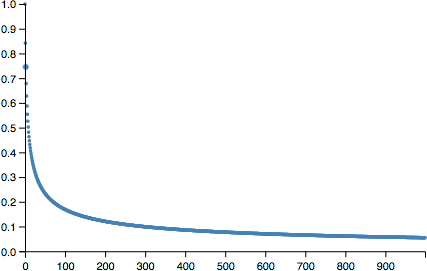
\includegraphics[scale=0.65]{convergence-sinx-double.png}
\caption{The iteration of $F(x_n)$ visually appears to converge.}
\end{figure}

We have the function $F(x_n) = \sin x_n = x_{n+1}$ and we want to know if it converges such that $\sin \alpha = \alpha$ where $\alpha$ is a fixed point of the iteration $F(x_n)$.

We know that a function has a fixed point if it intersects with the identity function $x = y$ in a specified interval. Consider $g(x) = \sin(x) - x = 0$ on the interval $[-1, 1]$. At the left bounds $x = -1$ we have $g(-1) > 0$, and at the right we have $g(1) < 0$, thus by the intermediate value theorem we know that it must have a root in the interval $[-1, 1]$. Therefore there exists a value of $x$ such that $\sin x = x$ within this interval. It's also obvious that $x = 0$ is the fixed point such that $\sin x = x$.

\begin{figure}[H]
\centering
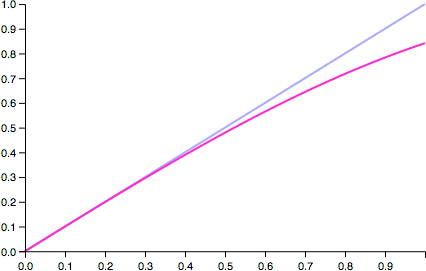
\includegraphics[scale=0.65]{sinx-xy-plot.png}
\caption{$\sin x = y$ crosses the function $x = y$ at $x = 0$, which is a fixed point of $\sin(x)$.}
\end{figure}

The derivative of $\sin^\prime x = \cos x$ is between $[0, 1]$ on the
interval $x \in [0,1]$. So $\sin x$ is a monotone decreasing function
on this interval and we know that it has no other fixed points and
must converge to $0$. Therefore iterating from $x_0 = 1$ will
eventually converge to $0$.

With Newton's method the convergence of $F(x_n)$ is very slow. The
value for the Newton's step $\frac{F(x)}{F^\prime(x)}$ becomes very
small as we move closer to $0$ from above, becuase the rate of change
approaches $1$. This can be seen visually
as the curve for $F(x)$ gets very close to $x = y$ but only touches it
at $x=0$. For example, when coded with double precision, after
$100000$ iterations we arrived at $x=0.00547696985405864$. Successive
iterations would continue to decrease, but would do so slower and slower.
}

\begin{minted}[mathescape,
               linenos,
               numbersep=5pt,
               gobble=2,
               framesep=2mm]{clojure}
  (first (drop 100000 (iterate #(Math/sin %) 1)))
  => 0.00547696985405864
\end{minted}
{\color{blue}

As the iteration converges we will have to deal with very small and
precise numbers. The precision of these numbers will quickly grow
beyond the bounds of traditionaly floating point or double arithmetic
operations. It's possible that trying to converge to $0$ may never
go below a precise threshold, or may skip around $0$ with once the
iteration of $F(x_n)$ becomes arbitrarily small.

}
